\documentclass[11pt]{article}
\usepackage{icmlko}
\begin{document}

\title{십오 년 전 완결작 835편이 판을 올렸다 --- 그리고 위약이 그것을 지웠다}
\author{월드모델 실험실}
\date{노트 387 · 2026년 8월 1일}
\maketitle

\begin{abstract}
노트 383이 웹툰 수집을 세어 보고 \texttt{title\_ids} 의
\texttt{range(1, 60)} 과 \texttt{len(fin) >= half} 조기 중단 때문에 플랫폼
3,827편 중 2,817편(74\%)만 갖고 있다는 것을 찾았다. 그때 ``빠진 26\%가
같은 분포라 급하지 않다''고 적었는데, \textbf{급하지 않다는 것과 값이
없다는 것은 다르다.} 웹툰은 무게 711로 판에서 제일 무거운 도메인이다.

빠진 것 중 835편을 받았다 --- 전부 2025년 이전(2005\,--\,2020)이라
\textbf{학습에만} 들어가고 \textbf{유보 711행은 두 팔이 같다}(노트 378
조항 ④). 웹툰 학습이 $2{,}106 \to 2{,}941$ 이 된다.

\begin{center}
\textbf{판 $0.4355 \to 0.4423$ · 웹툰 $+0.4543 \to +0.4977$} \\
짝 12뽑기 판 $\mathbf{+0.0071}$ (SD 0.0052) · \textbf{11/12} · 웹툰
$+0.0305$ · \textbf{12/12}
\end{center}

부호가 11/12 라 노트 378 조항 ①로 \textbf{판이 직접 채택}하고, 조건 ②도
만족한다(제일 나쁜 것이 도서 $-0.0219$, $t=-0.64$).

\textbf{그런데 위험 점검에서 하나가 걸렸다.} 옛 행의 축 넷은 100\% 그대로인데
\texttt{venue\_prominence} 만 82\% 다 --- 그 축이 표본 안 백분위라 행을
더하면 옛 행 값이 따라 움직인다. \textbf{그러면 이 이득이 새 자료 때문인지
눈금이 다시 매겨져서인지 모른다.} 갈랐다.

\begin{center}
\begin{tabular}{lrrrr}
\hline
갈래 & 판 차 & 부호 & 웹툰 차 & 부호 \\
\hline
① 그대로 & $+0.0071$ & 11/12 & $+0.0305$ & 12/12 \\
② 그 축을 양쪽 다 막고 & $+0.0065$ & 11/12 & $+0.0258$ & 11/12 \\
③ \textbf{새 행 라벨만 섞어서} & $+0.0011$ & 8/12 & $\mathbf{-0.0024}$ & 6/12 \\
\hline
\end{tabular}
\end{center}

\textbf{눈금은 8\%만 설명하고, 위약은 이득을 통째로 지운다.} 행 수가 늘어서
좋아진 것이 아니라 \textbf{그 835편의 라벨이 말하는 것} 때문이다.

새 챔피언: \textbf{판 0.4423 · 분모 3,430 · 웹툰 +0.4977 · 학습 2,941.}
웹툰 덮음은 74\%에서 95\%가 됐다.
\end{abstract}

\section{왜 이것을 골랐나}

노트 386의 남은 것 표에서 값이 제일 큰 항목은 ``왜 어디선 축이 통하나''
였는데, 설계를 넷 시도해 넷 다 떨어졌다(빈칸형은 이미 배제 · 라벨 알갱이는
안 갈림 · 라벨 축 구간 훑기는 좁히면 퍼짐이 같이 죽어 자기를 무너뜨림 ·
다른 축 가르기는 심슨 뒤집힘). \textbf{질문을 바꿨다.}

남은 것 중 실제로 잴 수 있는 제일 큰 항목이 웹툰이었다 --- 무게 711로
판의 21\%인데 덮음이 74\%다. 노트 381이 펀딩에서 학습을 넓혀
$+0.0322$(12/12)를 얻은 것과 같은 자리다.

\begin{figure}[t]
\centering
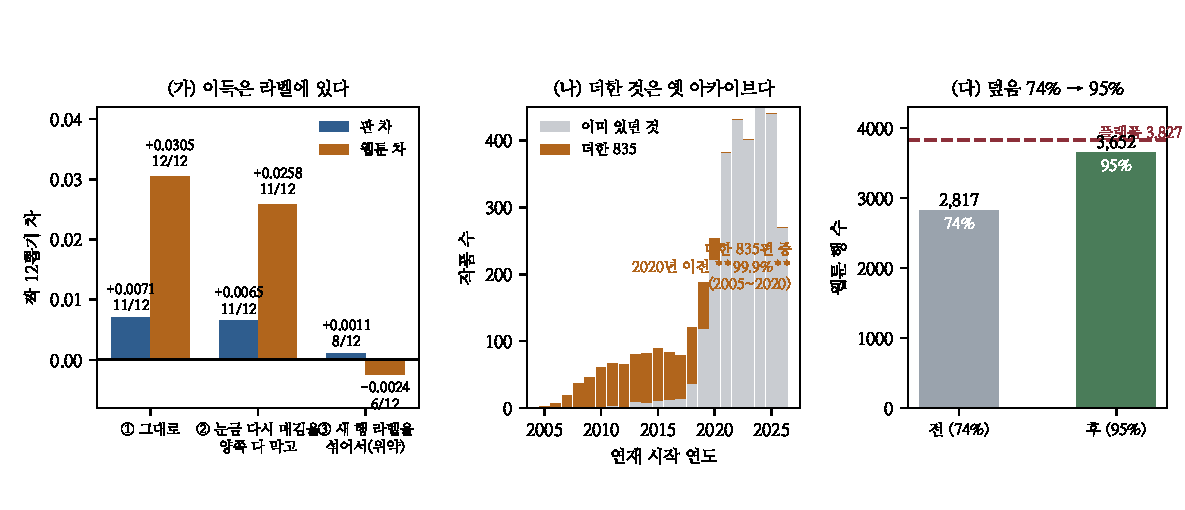
\includegraphics[width=\linewidth]{figs/fig387.pdf}
\caption{\textbf{(가)} 세 갈래의 짝 12뽑기 차. 눈금을 막아도 이득이 남고
(②), 라벨을 섞으면 사라진다(③). \textbf{(나)} 더한 835편의 연재 시작
연도 --- 99.9\%가 2020년 이전이다. \textbf{(다)} 덮음 74\% $\to$ 95\%.}
\label{fig:main}
\end{figure}

\section{쟀다}

\textbf{수집.} 노트 383이 만든 목록(플랫폼 3,827 $-$ 우리 2,817)에서
\texttt{webtoon\_domain.build} 를 그대로 써서 835편을 받았다. 원본 함수를
쓴 이유는 레코드 열 열여덟 개(\texttt{age\_rank} · \texttt{artists} ·
\texttt{star} · \texttt{level} $\ldots$)를 손으로 다시 맞추면 틀리기
때문이다 --- 처음에 손으로 짰다가 열이 안 맞아 버렸다.

\textbf{받은 것이 전부 옛 작품이다.} 2005\,--\,2020년이 834편, 2023년이
1편이다. \texttt{finished?order=UPDATE} 로 도는 아카이브의 꼬리라
\emph{갱신이 제일 오래된} 것들이고, 그것이 곧 옛 완결작이다. 그래서
\textbf{2025년 이후가 한 편도 없고, 유보가 안 바뀐다} --- 노트 378 조항
④(채점 집합이 다르면 잴 수 없음)를 자동으로 피한다.

\textbf{위험 점검.} 옛 2,817행의 라벨이 바뀐 행 0, 축은
\texttt{target\_breadth} · \texttt{entry\_friction} · \texttt{media\_push} ·
\texttt{goods\_scale} 이 100\% 그대로인데 \texttt{venue\_prominence} 가
82\% 다.

\section{갈랐다 --- 셋 중 하나만 남는다}

\textbf{① 그대로} 판 $+0.0071$ · 11/12. 첫 수치다.

\textbf{② 눈금 다시 매김을 뺀다.} \texttt{venue\_prominence} 를 두 팔에서
같이 막고 다시 재면 $+0.0065$ · 11/12 다. \textbf{이득의 92\%가 남는다}
--- 백분위가 밀린 것은 원인이 아니다. (막는 것이 옳은 대조인 이유는 노트
371 이다: 같은 실험 안에서 견줘야 한다.)

\textbf{③ 위약 --- 새 행의 라벨만 섞는다.} 835편을 그대로 넣되 그 라벨을
자기들끼리 뒤섞는다. 행 수 · 축 · 시대 분포가 전부 같고 \emph{라벨이
어느 작품 것인지}만 달라진다. 결과는 판 $+0.0011$(8/12) · 웹툰
$\mathbf{-0.0024}$(6/12) --- \textbf{이득이 통째로 사라진다.}

\textbf{그래서 이득은 ``행이 많아서''가 아니라 ``그 라벨이 맞아서''다.}
노트 133이 첫 양수를 그대로 채택하지 말라 한 것의 정석적인 자리이고,
이번에는 위약이 지워 주는 쪽이라 채택할 수 있다.

\section{왜 옛 완결작이 도움이 되나}

관측으로 둔다. 세 가지가 눈에 띈다.

\textbf{시대가 넓어진다.} 기존 학습은 2018년 이후가 대부분인데 더한 835편은
2005\,--\,2020이다. 노트 267이 ``모형의 우위는 날짜에서 안 온다''를 쟀으니
날짜 자체가 이득일 리는 없고, \emph{같은 축이 다른 시대에도 같은 방향인지}를
모형이 볼 수 있게 된 것으로 읽는다.

\textbf{완결작이라 축이 사후가 아니다.} 노트 263이 웹툰 \texttt{goods\_scale}
(회차 수)을 막은 이유가 ``연재 중 쌓인다''였는데, 완결작에서는 회차 수가
끝난 값이다. 다만 그 축은 지금도 막혀 있으므로 이 경로로는 안 들어온다.

\textbf{라벨 범위가 아래로 넓어진다.} 더한 835편에는 관심 수가 적은 옛
작품이 많다.

\textbf{셋 중 무엇인지 안 갈랐다} --- 노트 386에서 배운 대로, 네 점에 맞춘
곡선을 그리지 않는다. 가르려면 시대별로 나눠 넣어 보는 실험이 따로 필요하다.

\section{남은 것}

\begin{center}
\begin{tabular}{lll}
\hline
항목 & 왜 값이 큰가 & 어떻게 \\
\hline
웹툰 나머지 175편 & 덮음 95\% $\to$ 100\% · 2021\,--\,2026 & 수집이 멈췄다, 다시 돌린다 \\
어느 시대가 일했나 & 옛 작품 이득의 정체 & 835를 시대별로 나눠 넣어 본다 \\
같은 처방 다른 도메인 & 애니 606 · 모바일 441 도 덮음을 안 쟀다 & 노트 383 절차로 센다 \\
왜 어디선 축이 통하나 & 설계 넷이 떨어졌다 & 점을 늘리는 수밖에 \\
\hline
\end{tabular}
\end{center}

\end{document}
